\documentclass[11pt]{article}

\usepackage[portuguese]{babel}
\usepackage[utf8]{inputenc}
\usepackage{amsmath}
\usepackage{graphicx}
\usepackage{float}
\usepackage{subfig}
\usepackage{fixltx2e}
\usepackage[bottom]{footmisc}
\usepackage{color}
\usepackage[usenames,dvipsnames]{xcolor}
\usepackage[font=footnotesize]{caption}

\numberwithin{equation}{section}

\linespread{1.3}
\usepackage{indentfirst}
\usepackage[top=2cm, bottom=2cm, right=2.5cm, left=2.5cm]{geometry}
\addto\captionsportuguese{\renewcommand{\contentsname}{Índice}}

\begin{document}

\begin{titlepage}
\begin{center}

\hfill \break
\hfill \break


\includegraphics[width=0.3\textwidth]{./logo}~\\[1cm]

\textsc{\LARGE Instituto Superior Técnico}\\[0.25cm]
\textsc{\Large Mestrado Integrado em Engenharia Electrotécnica e de Computadores}\\[1.8cm]
\textsc{\huge Sistemas Integrados Analógicos}\\[0.25cm]

{\huge \bfseries Projecto de Alto Nível de um ADC e DAC \\[1cm]}

\begin{tabular}{ l l }
Maria Margarida Dias dos Reis & \hspace{2mm} n.º 73099 \\
Nuno Miguel Rodrigues Machado & \hspace{2mm} n.º 74236

\end{tabular}

\vfill

{\large Lisboa, 16 de Março de 2015} 

\end{center}
\end{titlepage}

\pagenumbering{gobble}
\clearpage

\tableofcontents
\pagebreak

\clearpage
\pagenumbering{arabic}

\section{Introdução}

Com este trabalho laboratorial pretende-se introduzir o \textit{software} Cadence, projectando um conversor AD/DA de alto nível. Analisando os conversores analógico-digitais (ADC) pode-se melhor compreender o conceito de \textit{Fast Fourier Transform} (FFT), e a maneira como pode ser aplicada para medir parâmetros dos ADC, como a SINAD e o ENOB. Pretende-se também estudar o efeito de aplicar diversas janelas sobre a FFT.

\section{Introdução Teórica}
\subsection{Conversores A/D e Conversores D/A}

Começando por analisar os conversores analógico-digitais, as arquitecturas que os permitem podem ser divididas em três categorias: baixa-a-média velocidade, média velocidade e alta velocidade. O ADC utilizado neste trabalho é de aproximações sucessivas (SAR), sendo de média velocidade e exactidão. 

Os conversores deste tipo estão entre os mais populares para realizar ADCs devido à sua versatilidade - conseguem efectuar conversões rápidas ou podem ser utilizados para que haja uma maior exactidão, operando a baixa potência nos dois casos. Este conjunto de características deriva de, no caso mais simples, o conversor necessitar apenas de um só comparador, um banco de condensadores com interruptores e pouca lógica de controlo digital. Na figura abaixo está esquematizado o circuito referido.

\begin{figure}[h]
	\centering
	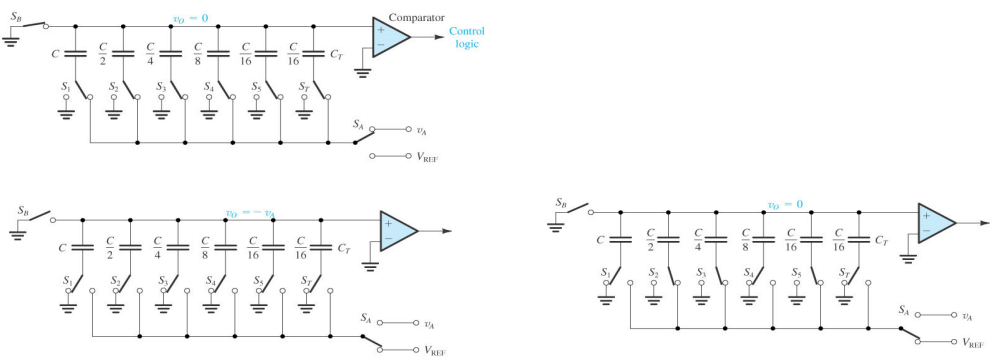
\includegraphics[keepaspectratio=true, scale=0.47]{./teoricas/SAR_1}
	\caption{ADC construído com uma arquitectura de aproximações sucessivas.}
	\vspace{-0.8em}
\end{figure}

O diagrama de blocos de um ADC unipolar de aproximações sucessivas que utiliza também um DAC é apresentado de seguida.
	
\begin{figure}[h]
	\centering
	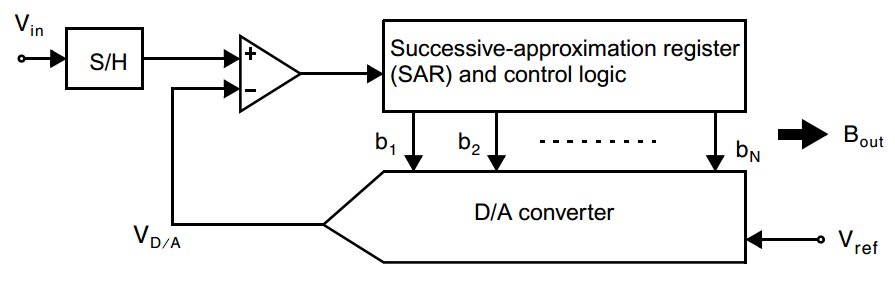
\includegraphics[keepaspectratio=true, scale=0.32]{./teoricas/SAR_2}
	\caption{Diagrama de blocos de um ADC de aproximações sucessivas.}
	\vspace{-0.8em}
\end{figure}

OS ADCs de aproximações sucessivas têm por base o algoritmo de procura conhecido como ``procura binária'', onde os dados podem ser calculados em $N$ passos, para um conjunto de dados organizados de tamanho $2^N$.

Existe um circuito \textit{sample-and-hold} que permite adquirir a tensão de entrada. De seguida um comparador analógico de tensão compara a tensão de entrada com a saída do DAC e coloca o resultado da comparação no registo de aproximações sucessivas (SAR). O SAR é inicializado de maneira a que o \textit{bit} mais significativo seja 1. Este código é dado ao DAC, que fornece então ao comparador uma tensão analógica equivalente à do código digital. O circuito comparador é assim capaz de efectuar a comparação entre a tensão de entrada amostrada e a tensão de referência. Se a tensão de referência for superior à tensão de entrada então é feito \textit{reset} ao \textit{bit}, passa a 0, caso contrário permanece a 1. 

De seguida, o próximo \textit{bit} é colocado a 1 e feito o mesmo teste, continuando esta ``procura binária'' até que todos os \textit{bits} tenham sido testados no SAR. Assim, o conversor aplica o algoritmo para determinar a palavra digital mais próxima que corresponde à tensão de entrada amostrada.

\subsection{SINAD, SNR, SFDR e ENOB}

O \textit{signal-to-noise and distortion} (SINAD) é uma medida da \textit{perfomance} dinâmica geral de um ADC. É o rácio entre a amplitude do sinal em \textit{root-mean-square} (valor eficaz) e o valor médio da \textit{root-sum-square} das restantes componentes espectrais, incluindo harmónicas, mas excluindo a componente DC. O cálculo do SINAD em $dB$ é feito de acordo com a expressão

\vspace{-3mm}
\begin{equation}
\text{SINAD} = 10\times \log_{10} \left(\frac{A^{2}_{\text{bin}(f_{in})}}{\sum_{n=2}^{\text{size}/2}\left(A^{2}_{n} - A^{2}_{\text{bin}(f_{in})}\right)}\right).
\label{eq:SINAD}
\end{equation}

\vspace{1mm}
O \textit{signal-to-noise ratio} (SNR) é calculado a partir dos dados da FFT, tal como a SINAD, mas as harmónicas do sinal são excluídas dos cálculos, deixando apenas os termos de ruído. De uma maneira mais abstracta pode ser descrito como a comparação entre o nível de sinal desejado ao nível de ruído. O cálculo do SNR, em $dB$, para um número $N$ de \textit{bits} é feito de acordo com a expressão

\vspace{-3mm}
\begin{equation}
\text{SNR} = 6,02N + 1,76.
\label{eq:SNR}
\end{equation}

\vspace{1mm}
A \textit{spurious free dynamic range} (SFDR) é o rácio entre a amplitude máxima do sinal a amplitude máxima seguinte, ou seja, é a diferença entre as duas amplitudes máximas. À semelhança da SINAD não inclui a componente DC. O cálculo da SFDR em $dB$ é feito de acordo com a expressão

\vspace{-3mm}
\begin{equation}
\text{SFDR} = 10\times \log_{10} \left(\frac{A^{2}_{\text{bin}(f_{in})}}{A^{2}_{\text{bin}_{\text{max}}(\neq f_{in})}}\right).
\label{eq:SFDR}
\end{equation}

\vspace{1mm}
O \textit{effective number of bits} (ENOB) é uma medida da resolução de um ADC. De facto, a resolução de um ADC é dada pelo número de \textit{bits} que são utilizados para representar um valor analógico porém, todos os ADCs reais introduzem ruído e distorção. Assim, o ENOB especifica o número efectivo de \textit{bits} que se tem na realidade, quando se considera a existência de ruído. O cálculo do ENOB é feito de acordo com a expressão

\vspace{-3mm}
\begin{equation}
\text{ENOB} = \frac{\text{SINAD}-1,76}{6,02}.
\label{eq:ENOB}
\end{equation}

\vspace{1mm}
No caso do trabalho laboratorial o ENOB é de 4 \textit{bits}.

De notar, que tratando-se de um ADC ideal que se está a estudar, os conceitos de SINAD e de SNR ``confundem-se'' pois não existe distorção.

\subsection{Janela Rectangular, Janela de Hamming e Janela de Blackman-Harris}

A FFT é um algoritmo que permite obter a \textit{Discrete Fourier Transform} (DFT) , sendo então uma análise que permite converter tempo para frequência. Quando se calcula a DFT a entrada é um sinal digital e a saída é a análise digital espectral desse sinal. Inerentes à DFT estão erros e, para mitigar esses erros, recorre-se a um processo denominado de \textit{windowing}.

A análise espectral da DFT depende de uma determinada frequência de amostragem, $f_{s}$, e, consequentemente, toda essa análise estará entre $0$ e metade de $f_{s}$. Assim, a largura de banda da DFT é proporcional ao ritmo de amostragem. Este período de amostragem é dado por

\vspace{-3mm}
\begin{equation}
\bigtriangleup t = \frac{1}{f_{s}},
\end{equation}

\vspace{1mm}
sendo que no domínio da frequência existem os chamados \textit{bins}. A frequência de um determinado \textit{bin} $k$ relaciona-se com a frequência do sinal de entrada de acordo com

\vspace{-3mm}
\begin{equation}
f_{k} = \frac{k}{N_{s} \bigtriangleup t},
\label{eq:freq_bin}
\end{equation}

\vspace{1mm}
onde $k$ corresponde ao número do \textit{bin}, que é sempre um inteiro, e $N_{s}$ ao número de amostras. Através de (\ref{eq:freq_bin}) pode-se deduzir qual é a máxima frequência que pode ser representada por um dado número de amostras.

\vspace{-3mm}
\begin{equation}
k = \frac{N_{s} f_{k}}{f_{s}}.
\label{eq:max_bin}
\end{equation}

\vspace{1mm}
Analise-se agora o caso do trabalho laboratorial, em que a onda de entrada tem uma frequência de 13,671875 kHz, a frequência de amostragem é de 1 MHz e são utilizadas 512 amostras. Espera-se que o máximo da amplitude ocorra em $k = 7$.

Ainda para o mesmo sinal de entrada, quando a frequência de amostragem passa para 1,1 MHz, espera-se que o máximo de amplitude ocorra em $k = 6,36364$. Este valor não é inteiro  e cada \textit{bin} corresponde a uma frequência e não a um intervalo de frequências. Assim sendo, a DFT não consegue representar energia em $k = 6,36364$ pelo que a energia tem uma \textit{leak} entre os \textit{bins} $k = 6$ e $k = 7$, fenómeno conhecido como \textit{spectral leakage}.

Para procurar resolver este problema de \textit{spectral leakage} existe \textit{windowing}. Com esse processo é possível concentrar a energia nos \textit{bins} que têm maior amplitude (os que estão próximos do \textit{bin} de amplitude máxima) e atenuar a energia dos \textit{bins} circundantes.

O \textit{windowing} é implementado multiplicando o sinal de entrada por uma função de janela. Existem diversas funções de janelas, considerando-se aqui a janela rectangular, a janela de Hamming e a janela de Blackman-Harris.

\begin{figure}[H]
	\centering
	\subfloat[]{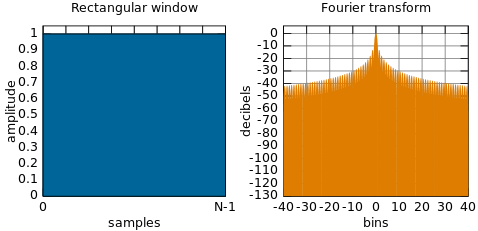
\includegraphics[keepaspectratio=true, scale=0.65]{teoricas/rectangular}}
	\linebreak
	\subfloat[]{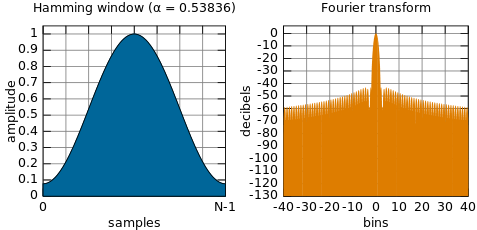
\includegraphics[keepaspectratio=true, scale=0.65]{teoricas/hamming}}
	\linebreak
	\subfloat[]{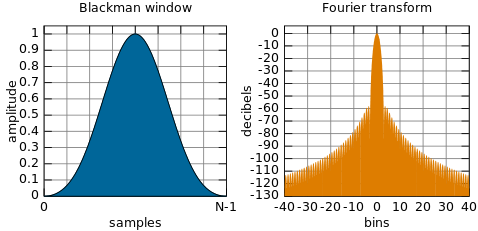
\includegraphics[keepaspectratio=true, scale=0.65]{teoricas/blackman}}
	\vspace{-0.8em}
	\caption{Magnitude (azul) e representação gráfica da DFT (laranja) da janela rectangular (a), magnitude (azul) e representação gráfica da DFT (laranja) da janela de Hamming (b) e  magnitude (azul) e representação gráfica da DFT (laranja) da janela de Blackman-Harris (c).}
	\vspace{-0.8em}
\end{figure}

\section{Demonstração de Resultados}

\subsection{Análise de uma onda sinusoidal com frequência de amostragem de 1 MHz}

Sabendo que se tem um frequência de amostragem, $f_{s}$, de 1 MHz e que a frequência do sinal de entrada, $f_{in}$, é de 13,671875 kHz, pode-se recorrer a (\ref{eq:max_bin}) para determinar qual é a máxima frequência que pode ser representada por um dado número de amostras, que neste caso é 512. Assim, verifica-se que $k$ é 7, tal como visto anteriormente, e nesse ponto espera-se um máximo de amplitude.

Uma vez que $k$ é um número inteiro, verifica-se coerência entre a frequência do sinal de entrada e a frequência de amostragem, pelo que pode-se dispensar o uso do processo de $windowing$ na FFT implementada.

Para que a FFT consiga reproduzir o sinal correctamente e sem distorção a partir das amostras obtidas é necessário que $k$ seja um número inteiro, e que a frequência de amostragem da FFT seja igual à frequência de amostragem do ADC. Como se utilizam $N_{s} = 512$ amostras e, sabendo que a frequência de amostragem do ADC é de $1$ MHz, para que a FFT tenha a mesma frequência de amostragem, aplica-se a fórmula 

\vspace{-3mm}
\begin{equation}
 	t_{\text{janela}} = \frac{N_{s}}{f_{s}},
 	\label{eq:temp_jan}
\end{equation}

\vspace{1mm}
que permite obter uma janela temporal, $t_{\text{janela}} = 512~\mu$s.

Com este valores definidos é então possível simular o circuito com o Cadence.

\begin{table}[h]
	\centering
	\caption{Valores obtidos para o ENOB, SINAD, SNR e SFDR com a janela rectangular.}
 	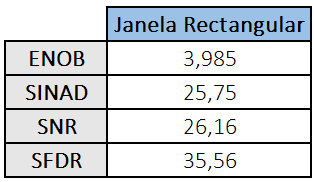
\includegraphics[keepaspectratio=true, scale=0.50]{lab/rect.png}
\end{table}

REFAZER TABELA COM UNIDADES, VERIFICAR SINAD E SNR

\begin{figure}[H]
	\centering
	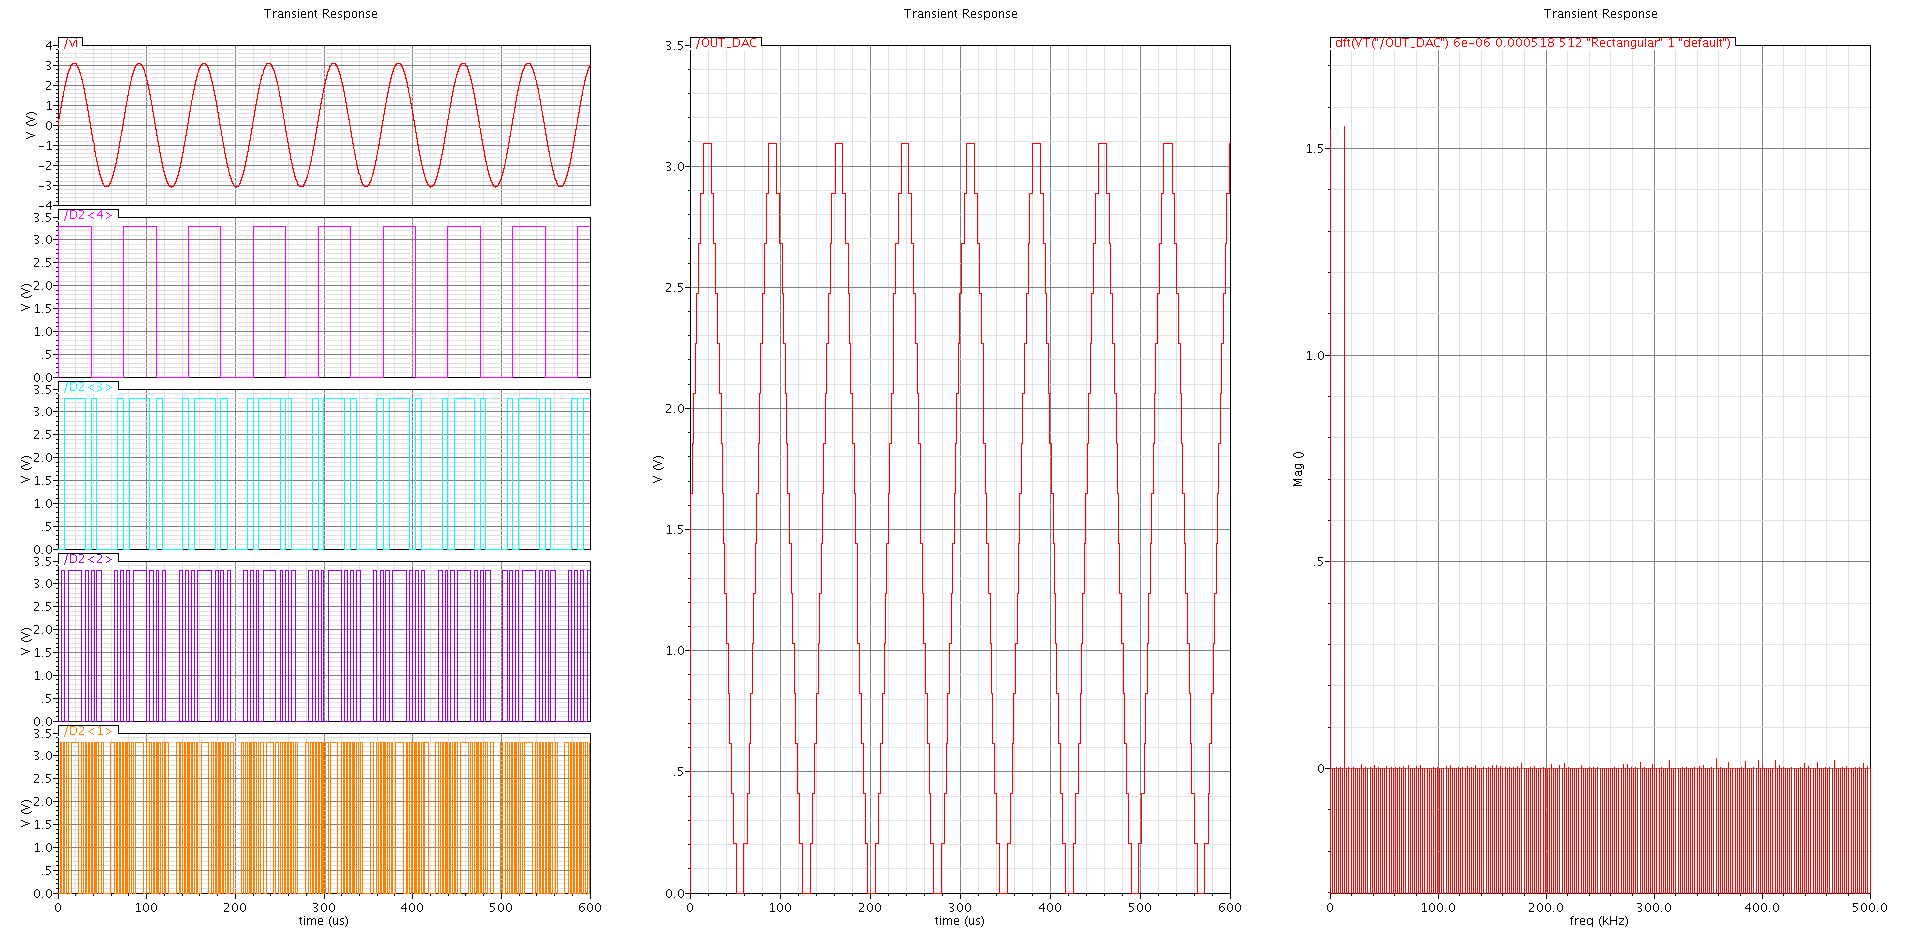
\includegraphics[keepaspectratio=true, scale=0.32]{lab/f_fft_1M.png}
	\caption{Simulação obtida no Cadence para o ADC para um valor de $f_{s}$ de 1 MHz.}
	\vspace{-0.8em}
\end{figure}
	 
Pode-se observar na Tabela 1 os resultados do ENOB, SINAD, SNR e SFDR calculados a partir da ferramenta de cálculo do Cadence. De notar que se obteve um valor de 3,985 \textit{bits} para o ENOB, valor que está muito próximo do pretendido, uma vez que se esta a utilizar um ADC ideal de 4 \textit{bits}.

O valor do SNR téorico pode ser calculado a partir de (\ref{eq:SNR}) e, sabendo que $N = 4$ \textit{bits}, dá um resultado de 25,84 dB. Para este caso o valor obtido foi de 25,75 dB, um resultado coerente com o número de \textit{bits} obtido para o conversor. 	 
	 
Na Figura 4, estão representados seis sinais no domínio temporal e um sinal no domínio da frequência. Pode-se visualizar o sinal sinusoidal de entrada, sinal à esquerda em cima, e os restantes quatro sinais representam a saída do ADC. No centro tem-se o sinal de saída do DAC. Por último, o sinal à direita, representa o espectro em frequência da FFT do sinal de saída do DAC.

No espectro de frequência pode-se visualizar graficamente as conclusões anteriormente referidas. Como o sinal de entrada é composto por uma frequência fundamental e existe coerência entre a frequência de amostragem e a de entrada, ocorre só um \textit{bin} na frequência do sinal de entrada, com amplitude correspondente a metade da amplitude do sinal de entrada, ou seja, 1,55 V.

e um \textit{bin} amostrado em DC. Mais ainda, verifica-se que não há distorção.

\subsection{Análise de uma onda sinusoidal com frequência de amostragem de 1,1 MHz}

Mantendo agora a mesma frequência para o sinal de entrada, $13,671875$ kHz, o mesmo número de amostras, $N_{s} = 512$, e alterando a frequência de amostragem para $1.1$ MHz, é refeita a análise relativamente ao ponto onde se espera que haja um máximo de amplitude da FFT. Recorrendo a (\ref{eq:max_bin}) obtém-se um valor de $k = 6,36364$, um valor que não é inteiro. 

Sabendo que este valor não é inteiro, sabe-se também que ocorre \textit{spectral leakage}, ou seja, a energia estará dispersa entre $k = 6$ e $k = 7$.

Para que a FFT consiga representar correctamente o sinal pretendido, é necessário definir um tamanho da janela correcto. Como já foi referido, a frequência de amostragem da FFT tem que ser igual à frequência de amostragem do sinal de entrada, ou seja de $1,1$ MHz com um número de amostras igual a 512. Assim, recorrendo a (\ref{eq:temp_jan}), obtém-se uma janela temporal, $t_{\text{janela}} = 465,455~\mu$s.

De notar que primeiramente foi feita uma simulação com a mesma janela temporal utilizada anteriormente, ou seja, com $t_{\text{janela}} = 512~\mu$s. Porém, com esta janela a FFT apresentava um \textit{bin} em $k = 7$, o que não correspondeu ao esperado de \textit{spectral leakage} e dispersão de energia. Desta maneira, alterou-se a janela e efectuaram-se novas simulações.

Com este valores definidos é então possível simular o circuito com o Cadence.

\begin{table}[H]
	\centering
	\caption{Valores obtidos para o ENOB, SINAD, SNR e SFDR com a janela rectangular, janela de Hamming e janela de Blackman-Harris.}
 	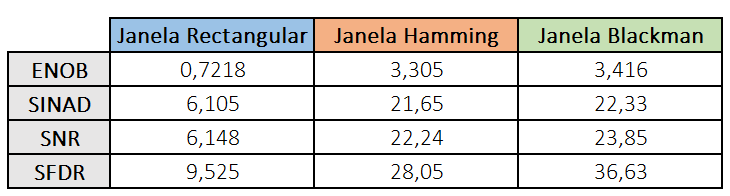
\includegraphics[keepaspectratio=true, scale=0.50]{lab/janelas.png}
\end{table}

REFAZER TABELA COM UNIDADES, VERIFICAR SINAD E SNR

\begin{figure}[H]
	\centering
	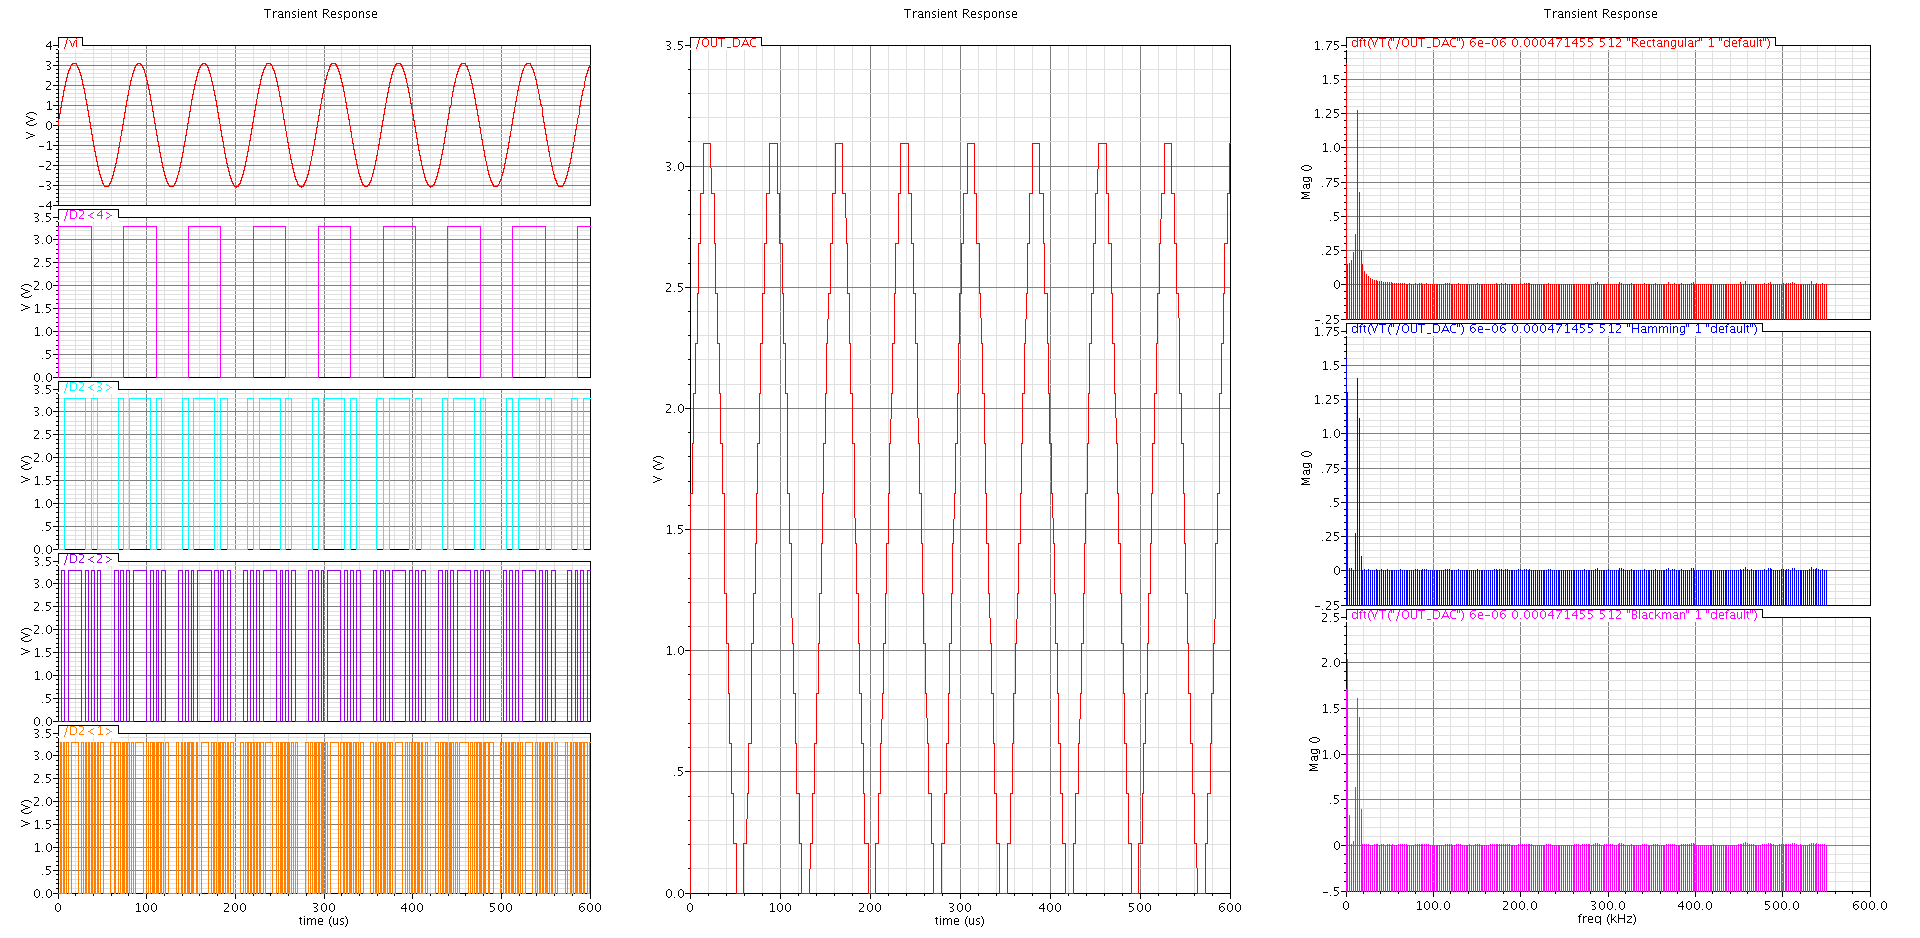
\includegraphics[keepaspectratio=true, scale=0.27]{lab/f_11M.png}
	\caption{Simulação obtida no Cadence para o ADC para um valor de $f_{s}$ de 1,1 MHz.}
	\vspace{-0.8em}
\end{figure}

\begin{figure}[H]
	\centering
	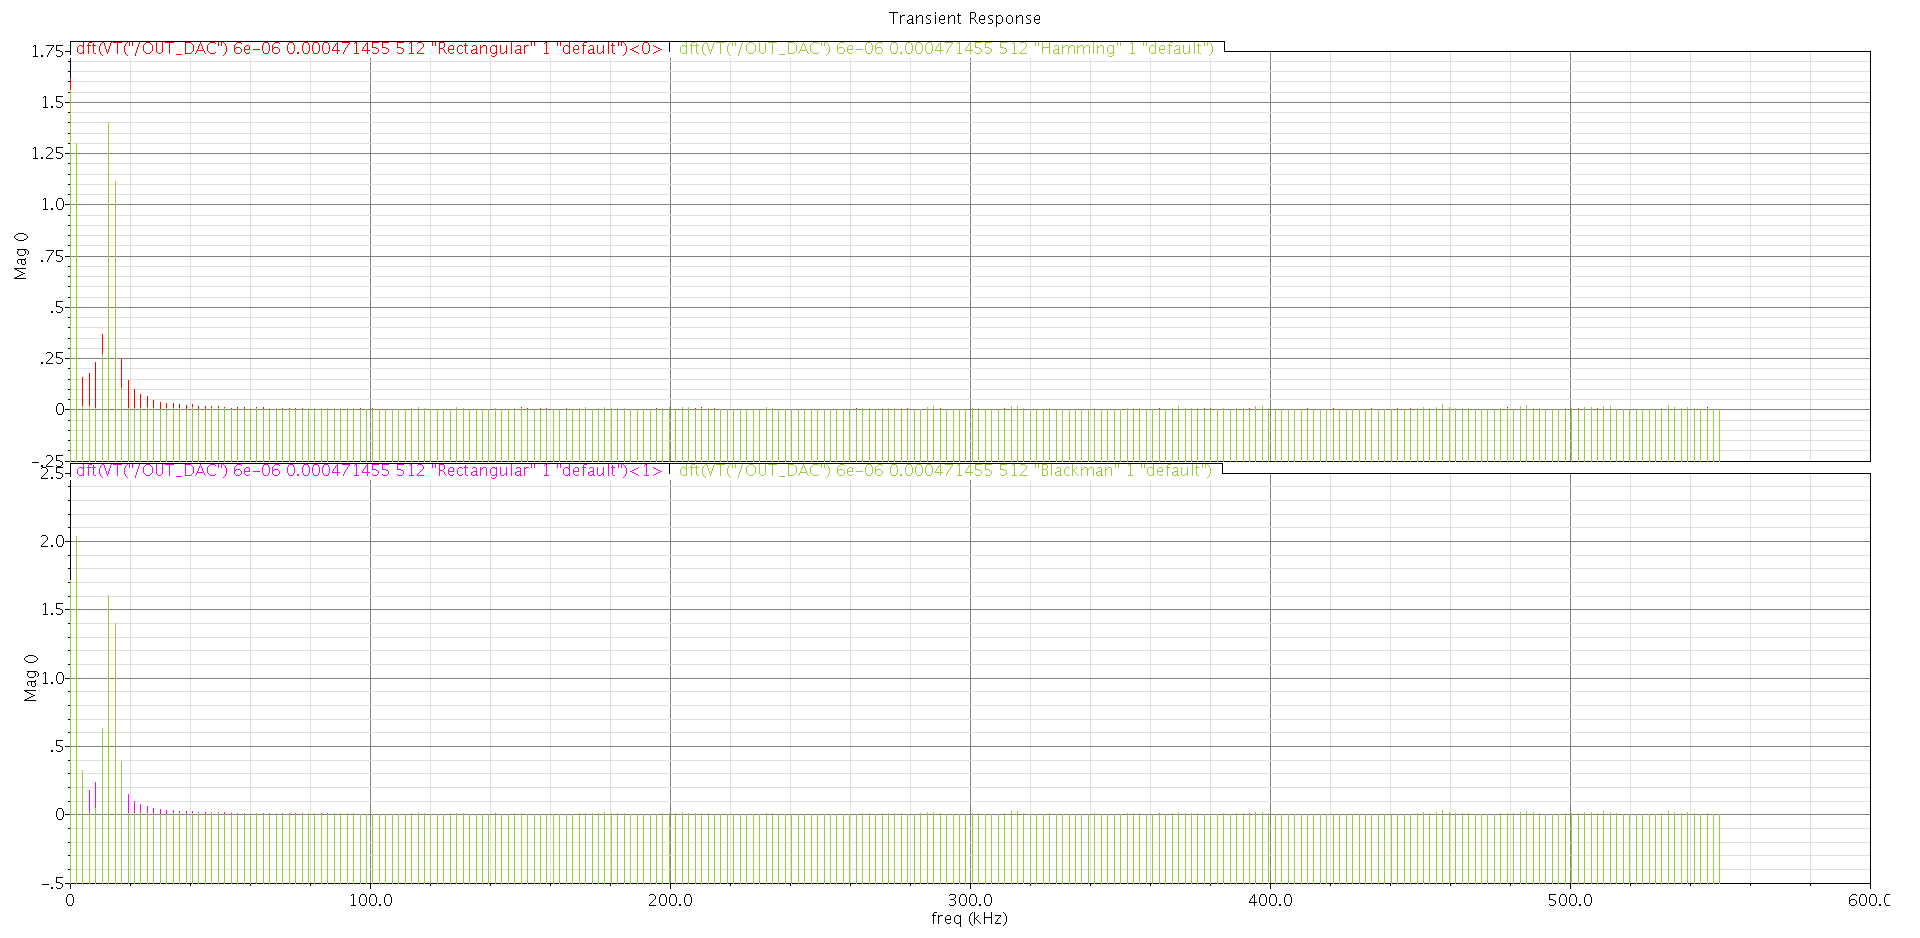
\includegraphics[keepaspectratio=true, scale=0.33]{lab/f_fft_11M.png}
	\caption{Simulação obtida no Cadence para a FFT, sobrepondo a janela rectangular com a de Hamming e de Blackman-Harris.}
	\vspace{-0.8em}
\end{figure}

Pode-se observar na Tabela 2 os resultados do ENOB, SINAD, SNR e SFDR calculados a partir da ferramenta de cálculo do Cadence, para o caso de aplicar sobre a FFT uma janela rectangular, a janela de Hamming e a janela de Blackman-Harris. Para o caso da janela rectangular, o número de \textit{bits} obtido foi de 0,7218, ou seja, um valor afastado do teórico de 4 \textit{bits}. Isto ocorre porque há \textit{spectral leakage}. 

Na Figura 5, à direita, observa-se o resultado da FFT com a aplicação de diversas janelas. Em cima, a vermelho, está o resultado com a janela rectangular, a azul, está o resultado com a janela de Hamming e a rosa, o resultado com a janela de Blackman-Harris. Analisando primeiramente a janela rectangular verifica-se que existe dispersão de energia, sendo o máximo de amplitude menor, passando de 1,55 V para 1,25 V. A janela rectangular tem o problema de todas as riscas espectrais terem a mesma ponderação, pelo que não consegue resolver o problema de \textit{spectral leakage}, sendo necessário aplicar outras janelas.

A ideia de aplicar outras janelas é tentar concentrar a energia em torno do \textit{bin} correspondente ao da frequência fundamental, ou seja, em torno do lóbulo principal da resposta em frequência da janela. Ao mesmo tempo, consegue-se atenuar a energia em torno dos \textit{bins} circundantes.

Primeiramente aplicou-se a janela de Hamming, e verifica-se na Tabela 2 que o ENOB passou para 3,305 \textit{bits}, um valor muito mais próximo do ideal. Comparativamente à janela rectangular, a resposta em frequência da janela de Hamming é mais concentrada no lóbulo principal, como se pode ver na Figura 3. Também nessa figura pode-se verificar que a janela de Blackman-Harris é ainda mais concentrada no lóbulo principal e atenua mais nos lóbulos secundários, ou seja, é mais selectiva. Isto pode ser comprovado pelo ENOB obtido para a janela de Blackman-Harris, que foi de 3,416 \textit{bits}, o mais próximo que se chegou dos 4 \textit{bits} ideais.

Relativamente à amplitude do \textit{bin} em torno de $k = 7$, esta aumenta da janela rectangular, com valor de 1,25 V, para a janela de Hamming, com valor superior a 1,25 V e mais próximo de 1,5 V. Quando se passa para a janela de Blackman-Harris, a amplitude já está a 1,5 V, tal como pretendido. Isto ocorre por causa da centralização de energia que o \textit{windowing} implica.

A melhoria introduzida pelo \textit{windowing} pode melhor ser observada na Figura 6. Em cima está a sobreposição entre a FFT obtida com janela rectangular, a vermelho, e com a janela de Hamming, a verde. Em baixo está a sobreposição entre a FFT obtida com janela rectangular, a vermelho, e com a janela de Blackman-Harris, a verde.

\section{Conclusões}


	 
\end{document}